\documentclass[a4paper, italian, oneside, 12pt]{article}
\usepackage[utf8x]{inputenc}
\usepackage[T1]{fontenc}
\usepackage[italian]{babel}
\usepackage{amsmath}
\usepackage{amssymb,amsfonts,textcomp}
\usepackage{array}
\usepackage{supertabular}
\usepackage{hhline}
\usepackage{fancyhdr}
\usepackage[version=3]{mhchem} 
\usepackage[bf, hang]{subfigure}
\usepackage[bf, hang]{caption}
\usepackage{graphicx}
\usepackage{float}
\usepackage[pdftex,pdfauthor={Ilario Gelmetti},pdfsubject={Study of some 2D NMR maps},pdfkeywords={NMR, COSY, ROESY, NOESY, difenilprolinolo},pdftitle={Relazioni di Laboratorio di Chimica Organica III},colorlinks=true,linkcolor=blue,citecolor=blue]{hyperref}
\setlength{\captionmargin}{.10\textwidth}
\usepackage{booktabs}
\usepackage{indentfirst}
\usepackage{lscape}
\usepackage{multicol}
\usepackage{wrapfig}

\newcommand\AlCentroPagina[1]{
\AddToShipoutPicture*{\AtPage{\bf{C$_{\textrm e}$}}nter{
\makebox(0,0){\includegraphics
[width=0.9\paperwidth]{#1}}}}}

\setlength{\headheight}{27pt} %se uso 12pt per il corpo testo, fancyhdr me lo chiede

\title{Relazioni di Laboratorio di Chimica Organica \romannumeral 3}
\author{Martina Bonciani, Beatrice De Nicola, Ilario Gelmetti, Andrea Leoncini}


\begin{document}

\setcounter{errorcontextlines}{\maxdimen}
%\frontmatter

\begin{titlepage}


\begin{center}
   	\large{\textsc{Facoltà di Scienze Matematiche Fisiche e Naturali}}\\
   	\large{{Dipartimento di Chimica e Chimica Industriale}}\\
    
		\rule{5cm}{1pt}\\
	\textsc{Anno Accademico 2010-2011}\\
			\makebox[\textwidth]{\rule{0pt}{.22\textheight}}\\
	\LARGE{\textsc{Relazioni di \\Laboratorio di Chimica Organica \romannumeral 3}}\\
	\bigskip	
		{\normalsize\makebox[.4\textwidth]{\rule{2cm}{1pt}}\\{Prof.$^{\rm{ssa}}$ Gloria Uccello Barretta}}\\
\end{center}

\vfill
\begin{small}
\makebox[\textwidth]{\rule{0pt}{.02\textheight}}\\
	\begin{center}
	\rule{3cm}{1pt}\\
	\large{Martina Bonciani, Beatrice De Nicola,\\ Ilario Gelmetti, Andrea Leoncini}\\		
	\end{center}
\end{small}


\end{titlepage}
\pagestyle{fancy}
\addtolength{\headwidth}{0.7cm}
\lhead[\fancyplain{}{\textbf{\footnotesize{\leftmark}}}]{}
\chead{}
\rhead[]{\fancyplain{}{\textbf{\footnotesize{\rightmark}}}}
\rfoot[\footnotesize{\slshape \footnotesize{\today}}]{\thepage}
\cfoot[\footnotesize{Relazioni di Laboratorio di Chimica Organica III}]{}
\lfoot[\thepage]{\footnotesize{\slshape Martina Bonciani, Beatrice De Nicola, Ilario Gelmetti, Andrea Leoncini}}

\tableofcontents
\makeatletter
\newcommand\arraybslash{\let\\\@arraycr}
\makeatother
\setlength\tabcolsep{1mm}
\renewcommand\arraystretch{1.3}

\newpage
\section{Composto A: (S)-2,2-difenil-prolinolo}

\begin{wrapfigure}{r}{0.28\textwidth}\vspace{-20pt}
  \begin{center}
    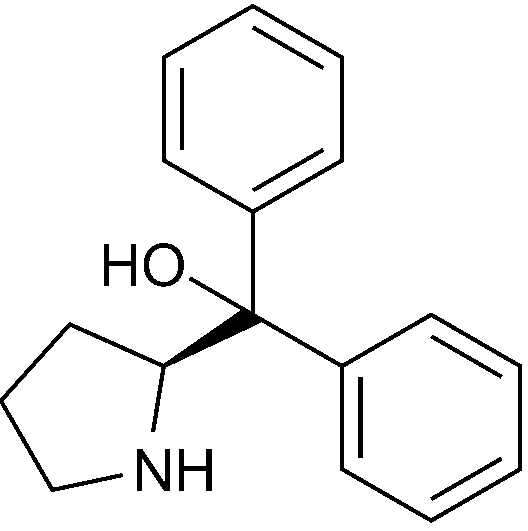
\includegraphics[width=0.26\textwidth]{img/A1.png}
  \end{center}\vspace{-20pt}
\end{wrapfigure}

\subsection{Breve panoramica degli spettri}

Nello spettro $^1$H si notano due gruppi di segnali: i protoni alifatici tra 1.5~ppm e 4.2~ppm, e i protoni aromatici tra 7.1~ppm e 7.6~ppm. Con la mappa TOCSY si evidenzia la separazione del sistema di spin alifatico dai due sistemi aromatici.

Tra 3 e 4~ppm si notano i segnali di tre protoni alifatici ben definiti e risolti.

Dall'integrazione dei segnali nello spettro $^1$H si individuano 17 protoni (7 alifatici, 10 aromatici) dunque gli idrogeni O--H e N--H non danno segnali ben definiti. Si può osservare un picco molto debole e allargato tra zero a 7~ppm, attribuibile al gruppo ossidrile.

\subsection{Assegnazione dei protoni alifatici}
\begin{wrapfigure}{r}{0.35\textwidth}\vspace{-20pt}
  \begin{center}
    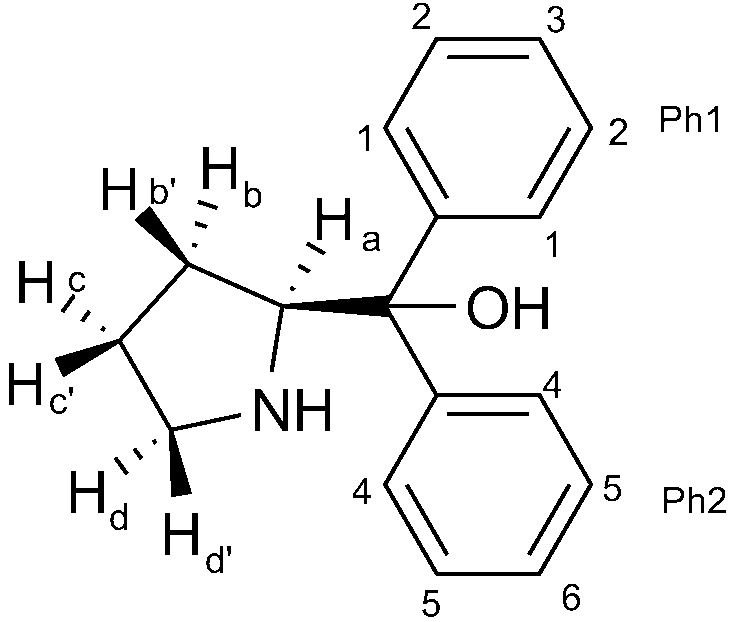
\includegraphics[width=0.33\textwidth]{img/A2.png}
  \end{center}\vspace{-20pt}
\end{wrapfigure}

Analizzando la mappa HSQC osserviamo che il protone più deschermato tra gli alifatici a 4.15~ppm è l'unico a dare un segnale positivo, quindi corrisponde ad {\bf{H$_{\textrm a}$}}, l'unico CH alifatico. Ulteriore conferma del fatto che si tratta di {\bf{H$_{\textrm a}$}} si ha dallo spettro $^1$H in cui si nota che il segnale integra per un solo protone. Possiamo quindi usarlo come protone sonda.

Dalla mappa COSY si individuano i protoni con cui accoppia {\bf{H$_{\textrm a}$}}: i due segnali a 1.59 e 1.66~ppm che corrispondono quindi uno a {\bf{H$_{\textrm b}$}} e l'altro a {\bf{H$_{b'}$}}. Questi ultimi mostrano a loro volta {\emph{cross peak}} con due segnali molto vicini tra loro a 1.74-1.75~ppm, che si possono quindi attribuire a {\bf{H$_{\textrm c}$}} e {\bf{H$_{\textrm c'}$}}. Da questi si seguono i {\emph{cross peak}} fino a identificare i protoni {\bf{H$_{\textrm d}$}} e {\bf{H$_{\textrm d'}$}} nei segnali ben risolti a 2.93~ppm e 3.02~ppm. 

Quindi dalla mappa HSQC si assegnano facilmente i segnali dei carboni alifatici, seguendo gli accoppiamenti con i rispettivi protoni.

L'assegnazione dei segnali dei protoni geminali è stata fatta sulla base della mappa ROESY: partendo dal segnale di {\bf{H$_{\textrm a}$}} si nota una forte interazione dipolare con il protone a 1.59~ppm, che quindi sarà {\bf{H$_{\textrm b}$}}, il protone spazialmente più vicino ad {\bf{H$_{\textrm a}$}}. Si osserva inoltre un'interazione debole con il protone a 2.93~ppm, che sarà pertanto {\bf{H$_{\textrm d}$}}. Per esclusione si assegnano i picchi di {\bf{H$_{\textrm b'}$}} a 1.66~ppm e {\bf{H$_{\textrm d'}$}} a 3.02~ppm. 

Partendo da {\bf{H$_{\textrm d}$}}, si osserva un {\emph{cross peak}} con il protone a 1.74~ppm, pertanto si assegna questo \emph{chemical shift} a {\bf{H$_{\textrm c}$}}. Analogamente, partendo da {\bf{H$_{\textrm d'}$}} si assegna il segnale a 1.75~ppm ad {\bf{H$_{\textrm c'}$}}.

Nello spettro $^1$H è interessante notare una particolarità dei segnali di {\bf{H$_{\textrm b}$}} e {\bf{H$_{\textrm b'}$}}: le intensità non rispettano il triangolo di Tartaglia, e si manifesta un certo effetto tetto. Questo accade perché i due protoni sono vicini come {\emph{chemical shift}} e fortemente accoppiati.

\subsection{Assegnazione dei protoni aromatici}

I segnali dei protoni aromatici si trovano tra 7.1~ppm e 7.6~ppm.

Usando la mappa ROESY si evidenzia la vicinanza spaziale di {\bf{H$_{\textrm a}$}} con i protoni aromatici che danno doppietti nello spettro $^1$H a 7.52~ppm e 7.59~ppm. 

Con la mappa TOCSY si evidenzia la presenza di tre sistemi di spin separati: uno alifatico e due aromatici. I due picchi dei protoni aromatici spazialmente vicini ad {\bf{H$_{\textrm a}$}} non danno accoppiamento tra di loro nella mappa TOCSY, quindi appartengono a due sistemi di spin separati: ognuno a uno dei due fenili.

Questi segnali si possono attribuire ai protoni \emph{orto} dei due gruppi fenilici. Si nota che il segnale a 7.59~ppm, tra i due, dà il picco ROESY più intenso con {\bf{H$_{\textrm a}$}}; il segnale a 7.52~ppm, d'altra parte, ha interazione dipolare anche con {\bf{H$_{\textrm b}$}}, ma non si osserva alcun {\emph{cross peak}} con {\bf{H$_{\textrm b'}$}}.

Partendo dai segnali dei protoni \emph{orto} e studiando i {\emph{cross peak}} si possono separare i segnali appartenenti ai due sistemi di spin. I segnali a 7.52~ppm, 7.29~ppm e 7.17~ppm appartengono a un fenile e i segnali a 7.59~ppm, 7.31~ppm e 7.18~ppm appartengono all'altro.

Sulla base della mappa ROESY, e con la conferma delle aree integrate dei segnali dello spettro $^1$H, assegniamo ai protoni \emph{meta} i segnali a 7.29~ppm e 7.31~ppm e ai protoni \emph{para} i segnali a 7.17~ppm e 7.18~ppm.

Dal fatto che tra i protoni \emph{orto} solo il protone a 7.52~ppm dia un picco ROESY con {\bf{H$_{\textrm b}$}} si deduce che i segnali a 7.52~ppm, 7.29~ppm e 7.17~ppm appartengono al fenile {\bf{1}} e i segnali a 7.59~ppm, 7.31~ppm e 7.18~ppm appartengono al fenile {\bf{2}}.

{%
\begin{table}

\begin{center}
\begin{tabular}{c|cccc}
\multicolumn{5}{c}{\bf{Parametri $^1$H NMR (600 MHz, \ce{CDCl3}, 25°C) del composto A}}\\\toprule
H & $\delta$ (ppm) & m  & J (Hz)& Integrazione\\\cmidrule(r){1-1}\cmidrule(l){2-5}
{\bf{H$_{\textrm a}$}}&4.15 & t&        $^3$J$_{a,b }$= $^3$J$_{a,b'}$= 7.7&1\\
{\bf{H$_{\textrm b}$}}&1.59 &m &-&1\\
{\bf{H$_{\textrm b'}$}}&1.66 & m &                   -&1\\
{\bf{H$_{\textrm c}$}}&1.74& m &                   -&1\\
{\bf{H$_{\textrm c'}$}}&1.75& m &                   -&1\\
{\bf{H$_{\textrm d}$}}&2.93 &dt&  $^3$J$_{d,c}$= $^3$J$_{d,c'}$= 7.4; $^2$J$_{d,d'}$= 9.3&1\\
{\bf{H$_{\textrm d'}$}}&3.02 &ddd& $^2$J$_{d',d}$= 9.3; $^3$J$_{d',c'}$= 6.9; $^3$J$_{d',c}$= 4.6&1\\
{\bf{H$_{\textrm 1}$}}  &7.52&dd &$^3$J$_{1,2}$= 8.5; $^4$J$_{1,3}$= 1.3&2\\
{\bf{H$_{\textrm 2}$}}  &7.29 &dd &       $^3$J$_{2,1}$= 8.5; $^3$J$_{2,3}$= 7.2&2 \\
{\bf{H$_{\textrm 3}$}}  &7.17 & dt&       $^3$J$_{3,2}$= 7.2; $^4$J$_{3,1}$= 1.3&1 \\
{\bf{H$_{\textrm 4}$}}  &7.59&dd &       $^3$J$_{4,5}$= 8.4; $^4$J$_{4,6}$= 1.3&2 \\
{\bf{H$_{\textrm 5}$}}  &7.31 &dd&       $^3$J$_{5,4}$= 8.4; $^3$J$_{5,6}$= 7.2&2 \\
{\bf{H$_{\textrm 6}$}}  &7.18&dt&       $^3$J$_{6,5}$= 7.2; $^4$J$_{6,4}$= 1.3&1 \\\bottomrule
\end{tabular}
\end{center}\end{table}

}%



\begin{figure}
\centering{\bf{Diagramma di assegnazione dei segnali $^1$H NMR di A.}\vspace{15pt}
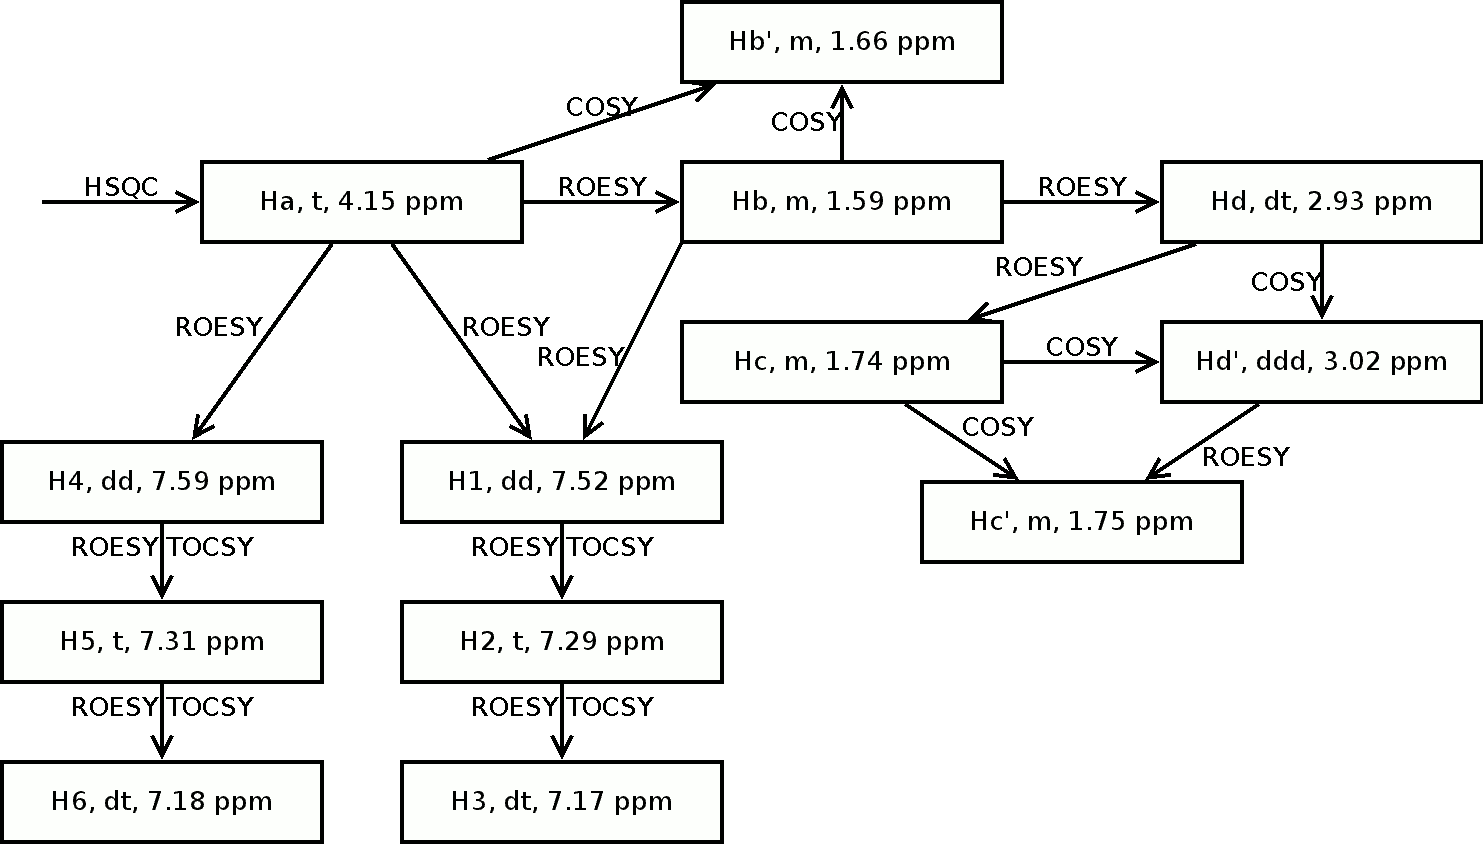
\includegraphics[width=1\textwidth]{img/compostoA.png}}
\vspace{-15pt}
\end{figure}

\subsection{Conformazione}

L'accoppiamento dei protoni \emph{orto} dei due fenili con il protone {\bf{H$_{\textrm a}$}} implica che l'ossidrile si trovi in posizione {\emph{anti}} rispetto ad {\bf{H$_{\textrm a}$}}. La vicinanza di un fenile a {\bf{H$_{\textrm b}$}} e la più alta intensità del {\emph{cross peak}} dell'altro fenile con {\bf{H$_{\textrm a}$}}, ci porta a dedurre una conformazione in cui il fenile {\bf{2}} è {\emph{sin-peri}} ad {\bf{H$_{\textrm a}$}} e il fenile {\bf{1}} si trova vicino ad {\bf{H$_{\textrm b}$}}. 

Sulla mappa ROESY si osservano le due interazioni dipolari di {\bf{H$_{\textrm a}$}} con {\bf{H$_{\textrm c}$}} e con {\bf{H$_{\textrm d}$}} essere più intense rispetto all'interazione tra {\bf{H$_{\textrm b'}$}} e {\bf{H$_{\textrm d'}$}} che a sua volta è più intensa di quella tra {\bf{H$_{\textrm b}$}} e {\bf{H$_{\textrm d}$}}. Dal primo dato deduciamo che {\bf{H$_{\textrm a}$}} sia in posizione pseudo-assiale. Le evidenze raccolte sono compatibili con una conformazione a busta dell'anello in cui {\bf{C$_{\textrm a}$}} stia fuori dal piano permettendo a {\bf{C$_{\textrm e}$}} di trovarsi in posizione pseudo-equatoriale. Questa conclusione è in accordo con la considerazione che essendo {\bf{C$_{\textrm e}$}} molto ingombrato questo debba trovarsi in posizione pseudo-assiale.


\subsection{Assegnazione dei carboni}


\begin{wrapfigure}{r}{0.35\textwidth}\vspace{-28pt}
  \begin{center}
    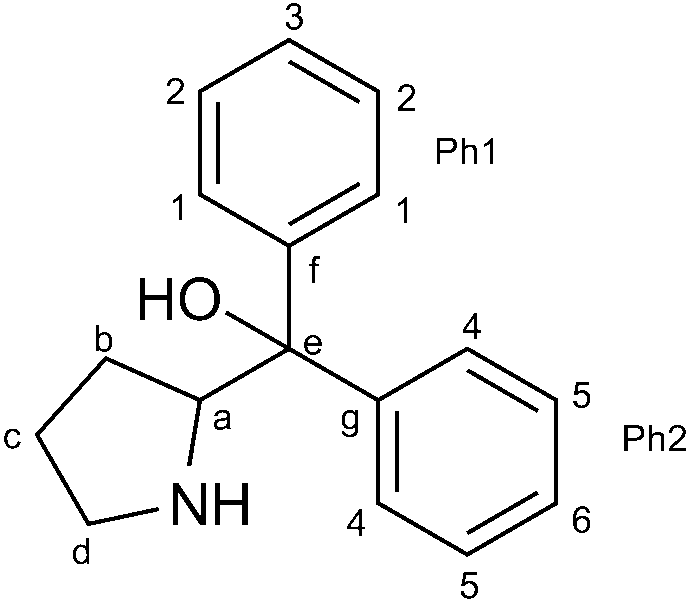
\includegraphics[width=0.33\textwidth]{img/A3.png}
  \end{center}\vspace{-20pt}
\end{wrapfigure}
Dallo spettro $^{13}$C si mette in evidenza il segnale del solvente \ce{CDCl3} (77~ppm) e la presenza di carboni aromatici e alifatici. Tra i segnali dei C alifatici se ne nota uno molto deschermato che, con la conferma dalla mappa HSQC, può essere attribuito a {\bf{C$_{\textrm a}$}}. Sempre dalla mappa HSQC, conoscendo gli spostamenti chimici dei protoni, si attribuiscono i {\emph{chemical shift}} agli altri carboni. Con l'impiego della mappa HMBC sono stati assegnati i {\emph{chemical shift}} dei carboni quaternari. Questi compaiono anche nello spettro $^{13}$C NMR, con intensità significativamente più bassa degli altri, poiché lo spettro è stato registrato in modalità {\emph{reverse}}.


{%
\begin{table}[hb]\begin{center}
 {\bf{Parametri $^{13}$C NMR (150 MHz, \ce{CDCl3}, 25°C) del composto A}}\end{center}

\begin{multicols}{2}
\begin{center}
\begin{tabular}{c|c}
\toprule
C & $\delta $ (ppm)\\\cmidrule(r){1-1}\cmidrule(l){2-2}
{\bf{C$_{\textrm a}$}} & 64.4\\
{\bf{C$_{\textrm b}$}} & 26.2\\
{\bf{C$_{\textrm c}$}} & 25.4\\
{\bf{C$_{\textrm d}$}} & 46.7\\
{\bf{C$_{\textrm e}$}} & 77.0\\
{\bf{C$_{\textrm f}$}} & 145.3\\
{\bf{C$_{\textrm g}$}} & 148.1\\\bottomrule
\end{tabular}
\end{center}
\columnbreak
\begin{center}
\begin{tabular}{c|c}
\toprule
C & $\delta $ (ppm)\\\cmidrule(r){1-1}\cmidrule(l){2-2}
{\bf{C$_{\textrm 1}$}} & 125.4\\
{\bf{C$_{\textrm 2}$}} & 127.9\\
{\bf{C$_{\textrm 3}$}} & 126.2\\
{\bf{C$_{\textrm 4}$}} & 125.7\\
{\bf{C$_{\textrm 5}$}} & 128.1\\
{\bf{C$_{\textrm 6}$}} & 126.4\\\bottomrule
\end{tabular}
\end{center}
\end{multicols}
\end{table}}

\clearpage


\section{Composto AOB: complesso B-metil-ossazaborolidina del (S)-2,2-difenil-prolinol-borano}

\begin{wrapfigure}{r}{0.30\textwidth}\vspace{-20pt}
  \begin{center}
    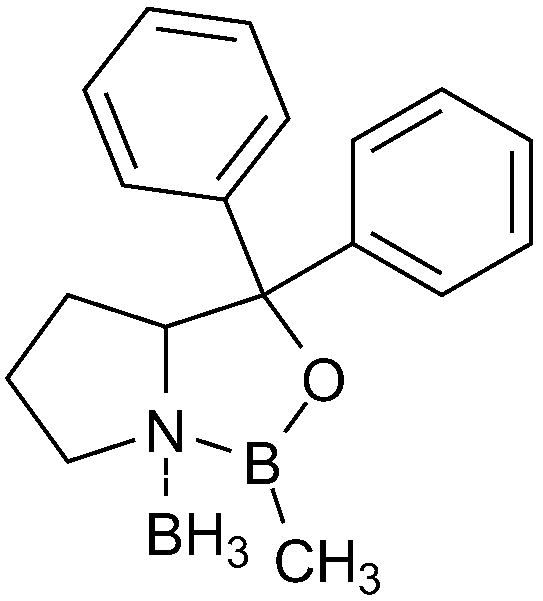
\includegraphics[width=0.27\textwidth]{img/AOB1.png}
  \end{center}\vspace{-20pt}
\end{wrapfigure}

\subsection{Breve panoramica degli spettri}
Nello spettro $^1$H si nota la presenza di molti segnali a bassa intensità facilmente distinguibili dai picchi intensi relativi alla molecola AOB; questi picchi sono attribuibili a impurezze. 

Dall'integrazione dei picchi principali nello spettro $^1$H si mette in evidenza un singoletto molto schermato che integra per tre protoni: è il metile legato all'atomo di boro ({\bf{B-CH$_{\textrm 3}$}}).

Dalla mappa TOCSY si può distinguere il sistema di spin alifatico dai sistemi aromatici. 
\subsection{Assegnazione dei protoni alifatici}


\begin{wrapfigure}{r}{0.41\textwidth}
  \begin{center}
    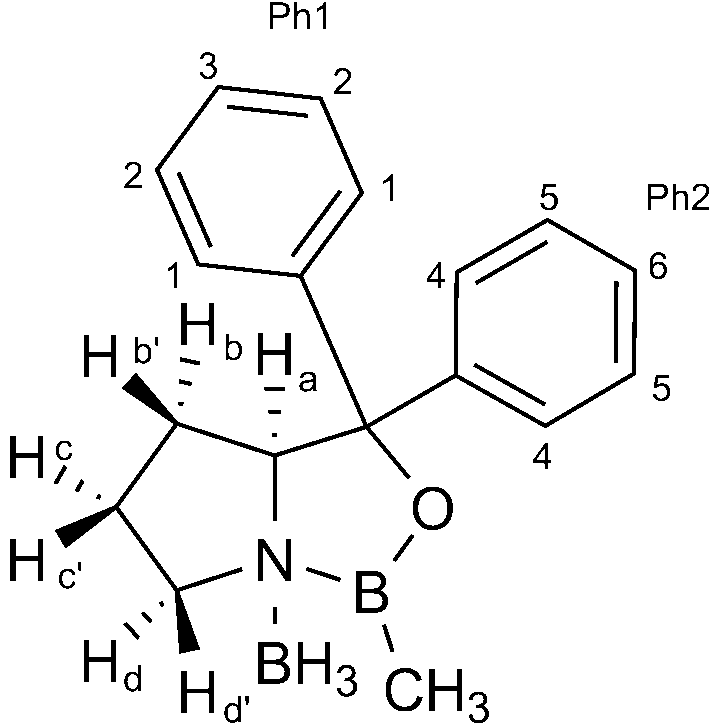
\includegraphics[width=0.38\textwidth]{img/AOB2.png}
  \end{center}
\end{wrapfigure}

Fra i segnali alifatici dello spettro $^1$H si nota la presenza di un tripletto molto deschermato integrante per 1 protone. Dalla mappa ROESY si trova che questo protone ha interazioni dipolari con gli aromatici e con un alifatico. Dunque questo picco deschermato si assegna ad {\bf{H$_{\textrm a}$}}.

Si scelgono i protoni {\bf{H$_{\textrm a}$}} e {\bf{B-CH$_{\textrm 3}$}} come sonde nell'investigazione delle mappe NMR.

Dalla mappa COSY, definiamo i {\emph{chemical shift}} dei multipletti alifatici a 1.16~ppm, 1.44~ppm, 1.77~ppm e 1.80~ppm, che non si distinguono bene dallo spettro $^1$H.

Nella mappa ROESY il protone {\bf{H$_{\textrm a}$}} ha interazione dipolare con il protone a 1.77~ppm, quindi questo è il segnale di {\bf{H$_{\textrm b}$}}. Il protone {\bf{H$_{\textrm a}$}} dà anche una interazione dipolare meno intensa con un segnale a 1.16~ppm che quindi è il segnale di {\bf{H$_{\textrm b'}$}}.

A causa di un segnale molto allargato fra 1~ppm e 2~ppm non è possibile riconoscere i {\emph{cross peak}} di accoppiamento fra i segnali di quest'area della mappa. Questo segnale \emph{broad} si può attribuire ai protoni del BH$_{\textrm 3}$ coordinato all'azoto. Risulta allargato a causa dei tempi di rilassamento brevi dei protoni legati al boro, dovuti al momento quadrupolare di quest'ultimo. 

Una volta ultimata l'assegnazione dei picchi presenti in questa regione, è possibile calcolare l'area del picco allargato per differenza tra l'area totale dei segnali e l'area corrispondente ai protoni assegnati in quella zona. Da tale calcolo risulta che al picco allargato corrispondono approssimativamente tre protoni; ciò conferma l'ipotesi iniziale (a meno di interferenze da parte di segnali di impurezze).

Procediamo all'assegnazione dei segnali partendo dai protoni sul metile legato al boro presente nell'anello. Questi protoni danno un picco ROESY intenso con il protone a 3.26~ppm. L'unico idrogeno che può dare questo segnale è {\bf{H$_{\textrm d'}$}}. Quest'ultimo protone mostra un picco ROESY molto intenso con il protone che risuona a 3.06~ppm, segnale pertanto attribuibile ad {\bf{H$_{\textrm d}$}}.
Questi due idrogeni hanno rispettivamente interazioni dipolari con i protoni a 1.44~ppm e a 1.80~ppm, che quindi sono il primo {\bf{H$_{\textrm c'}$}} e il secondo {\bf{H$_{\textrm c}$}}. 

L'analisi della mappa HSQC conferma la separazione in coppie geminali dei segnali protonici.

\subsection{Assegnazione dei protoni aromatici}

La mappa ROESY mostra che il protone {\bf{H$_{\textrm a}$}} è spazialmente vicino ai protoni fenilici a 7.47~ppm e a 7.24~ppm.

Il picco ROESY di {\bf{H$_{\textrm a}$}} con i protoni a 7.47~ppm è più intenso di quello coi protoni a 7.24~ppm, quindi questi ultimi si trovano più distanti. Possiamo attribuire i due segnali ai protoni \emph{orto} dei due sistemi aromatici. 

Con l'ausilio della mappa TOCSY si possono separare i segnali dei due sistemi di spin aromatici: il segnale a 7.47~ppm mostra accoppiamento con i segnali a 7.23~ppm e 7.13~ppm; per esclusione all'altro sistema aromatico appartengono i segnali a 7.24~ppm, 7.17~ppm e 7.08~ppm.

Nella mappa ROESY si nota {\emph{cross peak}} fra il protone {\bf{H$_{\textrm b}$}} e il protone a 7.24~ppm, ma non con il protone a 7.47~ppm. Quindi il sistema di spin composto dai segnali a 7.24~ppm, 7.17~ppm e 7.08~ppm appartiene al fenile {\bf{1}} e gli altri segnali aromatici appartengono al fenile {\bf{2}}.

Si osserva un picco ROESY tra il protone a 7.47~ppm e quello a 7.23~ppm che dunque assegniamo agli idrogeni \emph{meta} del fenile {\bf{2}}. Per esclusione il segnale a 7.13~ppm si assegna al protone \emph{para} del fenile {\bf{2}}. 

I protoni \emph{meta} e \emph{para} del fenile {\bf{1}} si assegnano in base all'area integrata nello spettro $^1$H-NMR: il segnale a 7.17~ppm appartiene ai protoni \emph{meta} mentre il segnale a 7.08~ppm appartiene al protone \emph{para}.
\vspace{30pt}


{%
\begin{table}
 \vspace{-25pt}
\begin{center}
\begin{tabular}{c|cccc}
\multicolumn{5}{c}{\bf{Parametri $^1$H NMR (600 MHz, \ce{CDCl3}, 25°C) del composto AOB}}\\\toprule
H & $\delta$ (ppm) & m  & J (Hz)& Integrazione\\\cmidrule(r){1-1}\cmidrule(l){2-5}
{\bf{H$_{\textrm a}$}} & 4.50 & t & $^3$J$_{a,b}$= $^3$J$_{a,b'}$= 8.0 & 1\\
{\bf{H$_{\textrm b}$}} & 1.77 & m & - & 1\\
{\bf{H$_{\textrm b'}$}} & 1.17 & m & - & 1\\
{\bf{H$_{\textrm c}$}} & 1.80 & m & - & 1\\
{\bf{H$_{\textrm c'}$}} & 1.45 & m & - & 1\\
{\bf{H$_{\textrm d}$}} & 3.06 & dt & $^2$J$_{d',d}$= 11.4; $^3$J$_{d,c'}$= $^3$J$_{d,c}$= 6.0 & 1\\
{\bf{H$_{\textrm d'}$}} & 3.26 & dt & $^3$J$_{d',c}$= $^3$J$_{d',c'}$= 7.3; $^2$J$_{d,d'}$= 11.4 & 1\\
{\bf{H$_{\textrm 1}$}} & 7.24 & m & -* & 2\\
{\bf{H$_{\textrm 2}$}} & 7.17 & dd & $^3$J$_{2,1}$= 8.4; $^3$J$_{2,3 }$= 7.3 & 2\\
{\bf{H$_{\textrm 3}$}} & 7.08 & t & $^3$J$_{3,2}$= 7.3 & 1\\
{\bf{H$_{\textrm 4}$}} & 7.47 & dd & $^3$J$_{4,5}$= 8.3; $^4$J$_{4,6}$=1.2 & 2\\
{\bf{H$_{\textrm 5}$}} & 7.23 & m & -* & 2\\
{\bf{H$_{\textrm 6}$}} & 7.13 & tt & $^3$J$_{6,5}$= 7.3; $^4$J$_{6,4}$=1.2 & 1\\
{\bf{B-CH$_{\textrm 3}$}} & 0.63 & s & - & 3\\\bottomrule
\end{tabular}
\end{center}\vspace{-10pt}
*i due segnali sono interamente sovrapposti.

\end{table}
}%


\begin{figure}
\centering{\bf{Diagramma di assegnazione dei segnali $^1$H NMR di AOB.}\vspace{5pt}
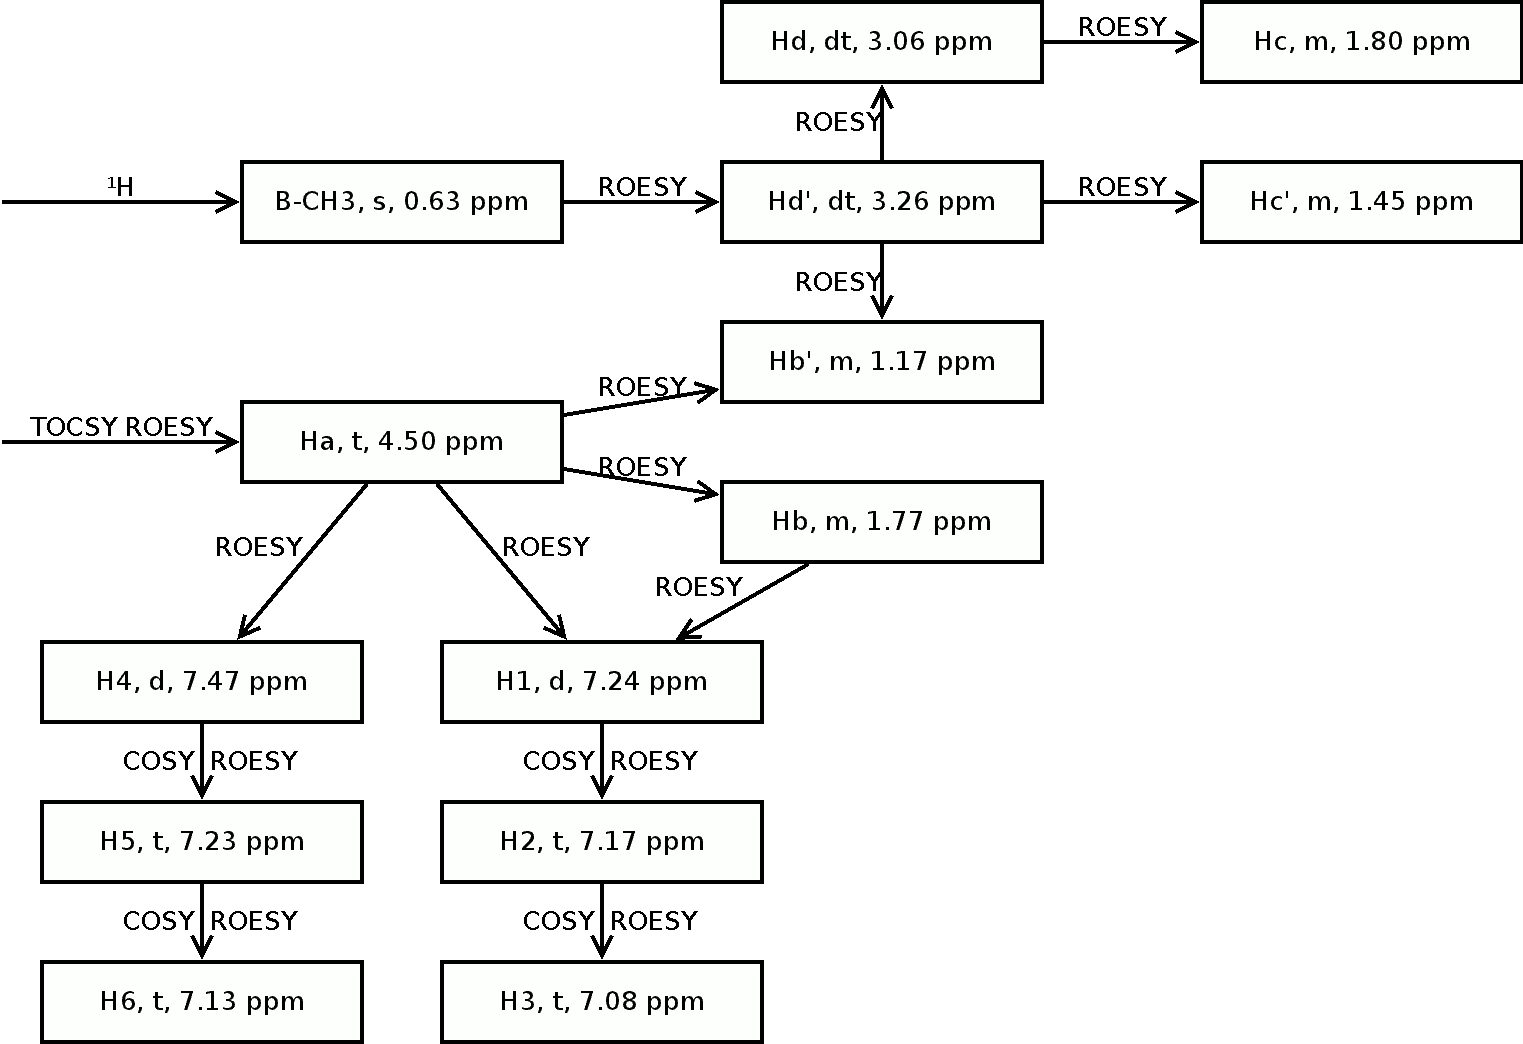
\includegraphics[width=1\textwidth]{img/compostoAOB.png}}\vspace{-20pt}
\end{figure}


\subsection{Conformazione}

Per quanto riguarda la conformazione del ciclo pirrolidinico si ottengono informazioni dalle interazioni dipolari di {\bf{H$_{\textrm d'}$}} osservabili sulla mappa ROESY. Questo protone mostra {\emph{cross peak}} di intensità leggermente maggiore con {\bf{H$_{\textrm b'}$}} che con {\bf{H$_{\textrm c}$}} dunque in questa conformazione la distanza tra {\bf{H$_{\textrm b'}$}} e {\bf{H$_{\textrm d'}$}} è simile alla distanza tra {\bf{H$_{\textrm c}$}} e {\bf{H$_{\textrm d'}$}}. Pertanto ipotizziamo una conformazione a busta in cui {\bf{H$_{\textrm c}$}} è pseudo-assiale e {\bf{H$_{\textrm c'}$}} è pseudo-equatoriale.

La conformazione prevalente del nucleo di ammonio quaternario si ricava osservando che l'intensità del picco ROESY di {\bf{B-CH$_{\textrm 3}$}} con {\bf{H$_{\textrm d'}$}} è più intenso di quello con {\bf{H$_{\textrm d}$}}. Perciò  il legante \ce{BH3} coordina l'azoto stando in posizione \emph{sin} rispetto ad {\bf{H$_{\textrm a}$}}. 

\subsection{Assegnazione dei carboni}

\begin{wrapfigure}{r}{0.30\textwidth}\vspace{-30pt}
  \begin{center}
    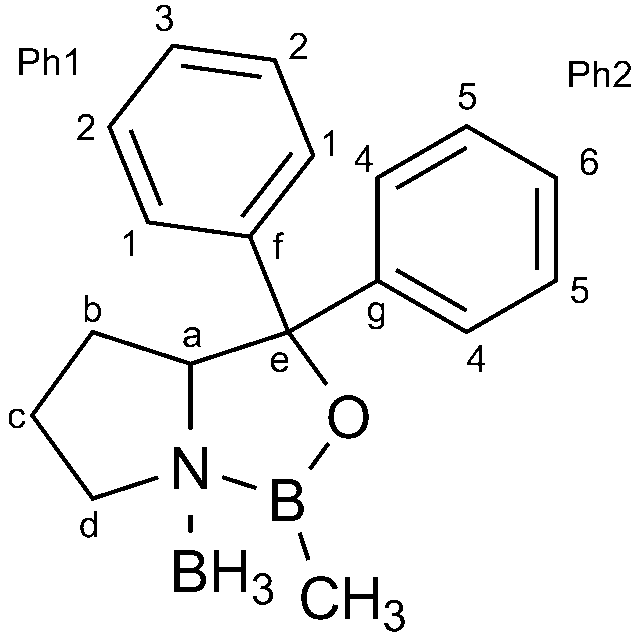
\includegraphics[width=0.28\textwidth]{img/AOB3.png}
  \end{center}\vspace{-27pt}
\end{wrapfigure}

Per l'assegnazione dei segnali $^{13}$C è stato necessario ricorrere all'impiego della mappa HMBC: nella HSQC i segnali non sono ben distinguibili, perciò risulta difficile dare una corretta attribuzione. Dal confronto tra la mappa HMBC e i {\emph{chemical shift}} protonici assegnati in precedenza, e tenendo conto degli accoppiamenti a lungo raggio, in particolar modo per i carboni quaternari, è stato possibile procedere con l'assegnazione di tutti i carboni. 
{%
\begin{table}[hb]\begin{center}
 {\bf{Parametri $^{13}$C NMR (150 MHz, \ce{CDCl3}, 25°C) del composto AOB}}\end{center}

\begin{multicols}{2}
\begin{center}
\begin{tabular}{c|c}
\toprule
C & $\delta $ (ppm)\\\cmidrule(r){1-1}\cmidrule(l){2-2}
{\bf{C$_{\textrm a}$}} &
 76.3\\{\bf{C$_{\textrm b}$}} &
 31.5\\{\bf{C$_{\textrm c}$}} &
 25.1\\{\bf{C$_{\textrm d}$}} &
 57.8\\{\bf{C$_{\textrm e}$}} &
 90.7\\{\bf{C$_{\textrm f}$}} &
 143.7\\{\bf{C$_{\textrm g}$}} &
 144.8\\\bottomrule
\end{tabular}
\end{center}
\columnbreak
\begin{center}
\begin{tabular}{c|c}
\toprule
C & $\delta $ (ppm)\\\cmidrule(r){1-1}\cmidrule(l){2-2}
{\bf{C$_{\textrm 1}$}} &
 128.4\\{\bf{C$_{\textrm 2}$}} &
 125.1\\{\bf{C$_{\textrm 3}$}} &
 127.2\\{\bf{C$_{\textrm 4}$}} &
 128.3\\{\bf{C$_{\textrm 5}$}} &
 125.5\\{\bf{C$_{\textrm 6}$}} &
 127.5\\{\bf{B-CH$_{\textrm 3}$}} &
 -5\\\bottomrule
\end{tabular}
\end{center}
\end{multicols}
\end{table}}



\clearpage

\section{Impurezza}
\subsection{Breve panoramica degli spettri}

Nello spettro e nelle mappe del composto AOB si osserva la presenza di una serie di segnali di intensità minore rispetto a quelli principali; si è quindi provato ad attribuire questi segnali a un altro composto presente in soluzione.

Dalla mappa ROESY si osserva un {\emph{cross peak}} negativo (dello stesso segno dei picchi sulla diagonale) di scambio tra {\bf{H$_{\textrm a}$}} di AOB e un protone a 4.26~ppm: possiamo attribuire questo segnale al protone corrispondente ad {\bf{H$_{\textrm a}$}} su una molecola in equilibrio chimico con AOB. 

In effetti si osserva che anche gli altri segnali dell'impurezza hanno dei picchi di scambio di segno negativo con i protoni nella molecola AOB. Da ciò confermiamo che l'impurezza presente nella mappa non è un precursore bensì una struttura in equilibrio con la molecola AOB.

Dallo spettro DOSY si riscontra solo una minima differenza tra il coefficiente di diffusione del composto AOB e quello dell'impurezza (quest'ultima ha un coefficiente di diffusione leggermente maggiore). Perciò si può escludere che l'impurezza sia una forma associata del composto AOB. Si può ipotizzare che l'impurezza sia un composto simile al composto AOB ma leggermente più leggero oppure meno solvatato.

Sulla base del rapporto tra l'area dei picchi dell'impurezza e dei corrispondenti picchi del composto AOB si deduce che il rapporto [impurezza]/[AOB] è pari a 0.13.

I protoni e i carboni su questa molecola verranno etichettati con i nomi dei corrispondenti protoni e carboni sulla molecola AOB.

A frequenze basse, nello spettro $^1$H-NMR, si osserva un singoletto a 0.29~ppm che integra per 3 protoni relativamente alle aree dell'impurezza, perciò possiamo attribuire questo picco ai protoni metilici di {\bf{B-CH$_{\textrm 3}$}} sull'impurezza.

Nello spettro $^1$H-NMR si osserva un singoletto a 2.09~ppm. Cercando questo segnale nelle mapppe non si trova nessun picco di accoppiamento di questo con altri. Osservando lo spettro DOSY (a cui è stata applicata una trasformata bayesiana) ci si rende conto che il segnale a 2.09~ppm appartiene a una molecola diversa da quelle analizzate e a cui corrisponde solo quel picco; probabilmente il residuo di un reattivo. Questa molecola si trova a coefficienti di diffusione maggiori delle altre.

Si osserva anche un altro singoletto a 0.00~ppm con le stesse caratteristiche del precedente a cui, nuovamente, non corrispondono altri picchi all'idrogeno però questa volta con un coefficiente di diffusione minore delle altre molecole: un'altra impurezza di scarso interesse.

\subsection{Assegnazione dei protoni alifatici}
La caratterizzazione dell'impurezza è iniziata prendendo come idrogeno sonda {\bf{H$_{\textrm a}$}} trovato (come riportato nella precedente sottosezione) a 4.26~ppm. 

Sulla mappa ROESY osserva la presenza di una interazione dipolare di {\bf{H$_{\textrm a}$}} con un protone a 2.93~ppm che si assegna a {\bf{H$_{\textrm d}$}}; con due protoni a 1.67~ppm (integra per 2 protoni) e con un protone a 1.50~ppm. Nella mappa COSY il segnale di {\bf{H$_{\textrm a}$}} accoppia con il picco a 1.50~ppm e il picco a 0.72~ppm.

In base a questi risultati si ricava che questi ultimi due picchi corrispondono uno a {\bf{H$_{\textrm b}$}} e uno a {\bf{H$_{\textrm b'}$}}. Questi danno anche accoppiamento con i protoni con {\emph{chemical shift}} a 1.67~ppm che sono quindi {\bf{H$_{\textrm c}$}} ed {\bf{H$_{\textrm c'}$}}. 

{\bf{H$_{\textrm d}$}} ha un picco di accoppiamento COSY a 3.38~ppm con {\bf{H$_{\textrm d'}$}} e un altro meno intenso con i protoni a 1.67~ppm.

Tornando alla mappa ROESY si osserva che il protone {\bf{H$_{\textrm a}$}} ha interazione dipolare più forte con il protone a 1.50~ppm che con quello a 0.72~ppm, si assegna pertanto quest'ultimo a {\bf{H$_{\textrm b'}$}} e il primo a {\bf{H$_{\textrm b}$}}.

Si notano dei {\emph{cross peak}} negativi (dello stesso segno della diagonale) nella mappa ROESY tra il segnale di {\bf{H$_{\textrm b'}$}} e quello a 1.17~ppm che era stato assegnato nella molecola AOB ad {\bf{H$_{\textrm b'}$}}.

Si ipotizza che {\bf{H$_{\textrm b'}$}} della molecola di “impurezza” si trovi a {\emph{chemical shift}} così bassi a causa dell'anisotropia magnetica del fenile {\bf{1}} causata dalla sua conformazione bloccata o dalla minore distanza media tra l'anello e {\bf{H$_{\textrm b'}$}}.

\subsection{Assegnazione dei protoni aromatici}
Nella mappa ROESY cercando le interazioni dipolari con i protoni aromatici si osserva un picco intenso tra {\bf{H$_{\textrm b'}$}} e i protoni a 7.25~ppm che si possono perciò identificare nei 2 protoni in \emph{orto} su un fenile che ipotizziamo essere il fenile {\bf{1}}. 

Un altro picco ROESY positivo si osserva tra {\bf{H$_{\textrm b'}$}} e i protoni a 7.44~ppm, che potrebbero corrispondere agli idrogeni {\bf{H$_{\textrm 4}$}} oppure {\bf{H$_{\textrm 2}$}}. 

Il protone {\bf{H$_{\textrm a}$}} mostra un picco ROESY intenso solamente con i protoni a 7.44~ppm. Quindi il picco a 7.44~ppm appartiene ai protoni \emph{orto} {\bf{H$_{\textrm 4}$}} e quello a 7.25~ppm ai protoni \emph{orto} {\bf{H$_{\textrm 1}$}}. Come conferma dell'assegnazione dei protoni \emph{orto} {\bf{H$_{\textrm 4}$}} si osserva che nello spettro protonico il picco a 7.44~ppm è un doppietto.\vspace{30pt}


{%
\begin{table}
\begin{center}
\begin{tabular}{c|cccc}
\multicolumn{5}{c}{\bf{Parametri $^1$H NMR (600 MHz, \ce{CDCl3}, 25°C) dell'impurezza}}\\\toprule
H & $\delta$ (ppm) & m  & J (Hz)& Integrazione\\\cmidrule(r){1-1}\cmidrule(l){2-5}



{\bf{H$_{\textrm a}$}} & 4,26 & dd & $^3$J$_{a,b}$= 9.7; $^3$J$_{a,b'}$= 5.8 & 1\\
{\bf{H$_{\textrm b}$}} & 1,50 & m & & 1\\
{\bf{H$_{\textrm b'}$}} & 0,72 & m & & 1\\
{\bf{H$_{\textrm c}$}}+{\bf{H$_{\textrm c'}$}} & 1,67 & m & & 2\\
{\bf{H$_{\textrm d}$}} & 2,93 & m & & 1\\
{\bf{H$_{\textrm d'}$}} & 3,24 & coperto & coperto & coperto\\
{\bf{H$_{\textrm 1}$}} & 7,25 & coperto & coperto & coperto\\
{\bf{H$_{\textrm 2}$}} & & & &\\
{\bf{H$_{\textrm 3}$}}  & & & &\\
{\bf{H$_{\textrm 4}$}} & 7,44 & d & $^3$J$_{4,5}$= 7.3 & 2\\
{\bf{H$_{\textrm 5}$}} & & & &\\
{\bf{H$_{\textrm 6}$}} & & & &\\
{\bf{B-CH$_{\textrm 3}$}} & 0,29 & s & & 3\\\bottomrule
\end{tabular}
\end{center}\end{table}

}%


\begin{figure}
\centering{\bf{Diagramma di assegnazione dei segnali $^1$H NMR dell'impurezza.}\vspace{15pt}
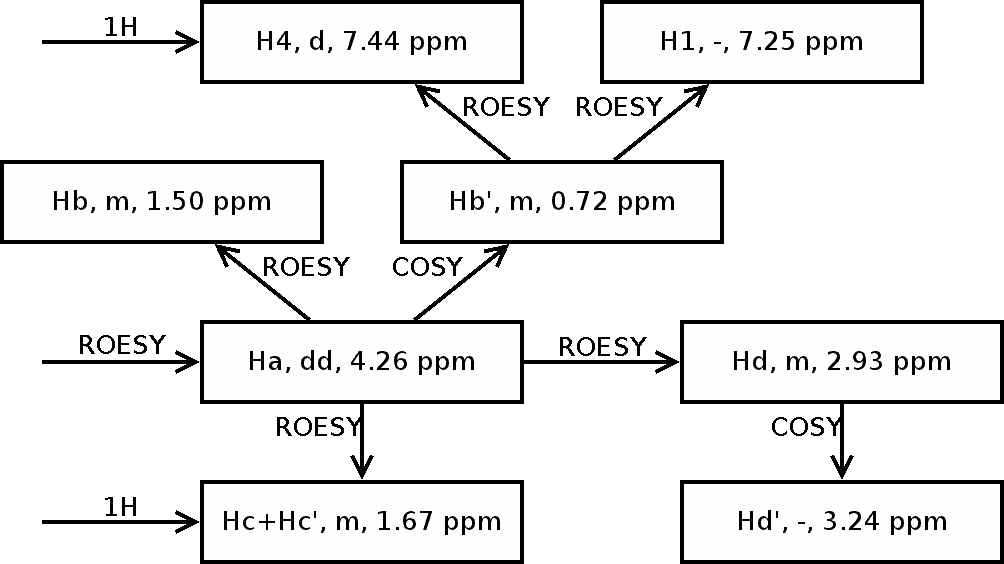
\includegraphics[width=0.8\textwidth]{img/impurezza.png}}\\
\vspace{-15pt}
\end{figure}

\subsection{Conformazione}
Si osservano le seguenti differenze in {\emph{chemical shift}} tra il composto AOB e l'impurezza in equilibrio con esso: i protoni {\bf{H$_{\textrm a}$}}, {\bf{H$_{\textrm b}$}}, {\bf{H$_{\textrm b'}$}}, {\bf{H$_{\textrm c}$}}, {\bf{H$_{\textrm d}$}}, {\bf{H$_{\textrm 4}$}} e {\bf{B-CH$_{\textrm 3}$}} si spostano a {\emph{chemical shift}} più bassi perciò sono più schermati; i protoni {\bf{H$_{\textrm d'}$}} e {\bf{H$_{\textrm 1}$}} non subiscono variazioni, il protone {\bf{H$_{\textrm c'}$}} viene spostato a {\emph{chemical shift}} più alti. 

Si può supporre che sia cambiata la conformazione dell'anello {\bf{C$_{\textrm a}$}} {\bf{C$_{\textrm b}$}} {\bf{C$_{\textrm c}$}} {\bf{C$_{\textrm d}$}} {\bf{N}} ma non si hanno sufficienti elementi per comprenderla.

Il generale spostamento verso frequenze basse potrebbe indicare che la molecola di impurezza non ha una parziale carica positiva sull'azoto ossia, a differenza della molecola AOB, non ha il BH$_{\textrm 3}$ complessante.

Dunque l'impurezza sarebbe la B-metil-ossazaborolidina del (S)-2,2-difenil-prolinolo.

Questa conclusione è compatibile con il coefficiente di diffusione leggermente maggiore osservato alla mappa DOSY.

Dai segnali della mappa ROESY si può supporre una struttura compatibile con una rotazione dei due fenili intorno al legame {\bf{C$_{\textrm a}$}}-{\bf{C$_{\textrm e}$}} probabilmente concomitante con una inversione dell'azoto.

\subsection{Assegnazione dei carboni}
Dallo spettro HSQC si ricavano i {\emph{chemical shift}} di {\bf{C$_{\textrm a}$}}, {\bf{C$_{\textrm b}$}}, {\bf{C$_{\textrm c}$}}, {\bf{C$_{\textrm d}$}}, {\bf{C$_{\textrm 4}$}} e {\bf{B-CH$_{\textrm 3}$}}.

{%
\begin{table}[ht]
\begin{center}

 {\bf{Parametri $^{13}$C NMR (150 MHz, \ce{CDCl3}, 25°C) dell'impurezza}}\end{center}

\begin{multicols}{2}
\begin{center}
\begin{tabular}{c|c}
\toprule
C & $\delta $ (ppm)\\\cmidrule(r){1-1}\cmidrule(l){2-2}

{\bf{C$_{\textrm a}$}} &
 72,6\\{\bf{C$_{\textrm b}$}} &
 30,2\\{\bf{C$_{\textrm c}$}} &
 26,2\\{\bf{C$_{\textrm d}$}} &
 42,8\\{\bf{C$_{\textrm e}$}} &
\\{\bf{C$_{\textrm f}$}} &
\\{\bf{C$_{\textrm g}$}} &\\\bottomrule
\end{tabular}
\end{center}
\columnbreak
\begin{center}
\begin{tabular}{c|c}
\toprule
C & $\delta $ (ppm)\\\cmidrule(r){1-1}\cmidrule(l){2-2}
{\bf{C$_{\textrm 1}$}} &
\\{\bf{C$_{\textrm 2}$}} &
\\{\bf{C$_{\textrm 3}$}} &
\\{\bf{C$_{\textrm 4}$}} &
 126,6\\{\bf{C$_{\textrm 5}$}} &
\\{\bf{C$_{\textrm 6}$}} &
\\{\bf{B-CH$_{\textrm 3}$}} &
 -5,4\\\bottomrule
\end{tabular}
\end{center}
\end{multicols}
\end{table}}

\clearpage
\renewcommand{\rightmark}{Spettri $^1$H NMR}

\addtolength{\hoffset}{-70pt}


\begin{landscape}
\begin{figure}[ht]
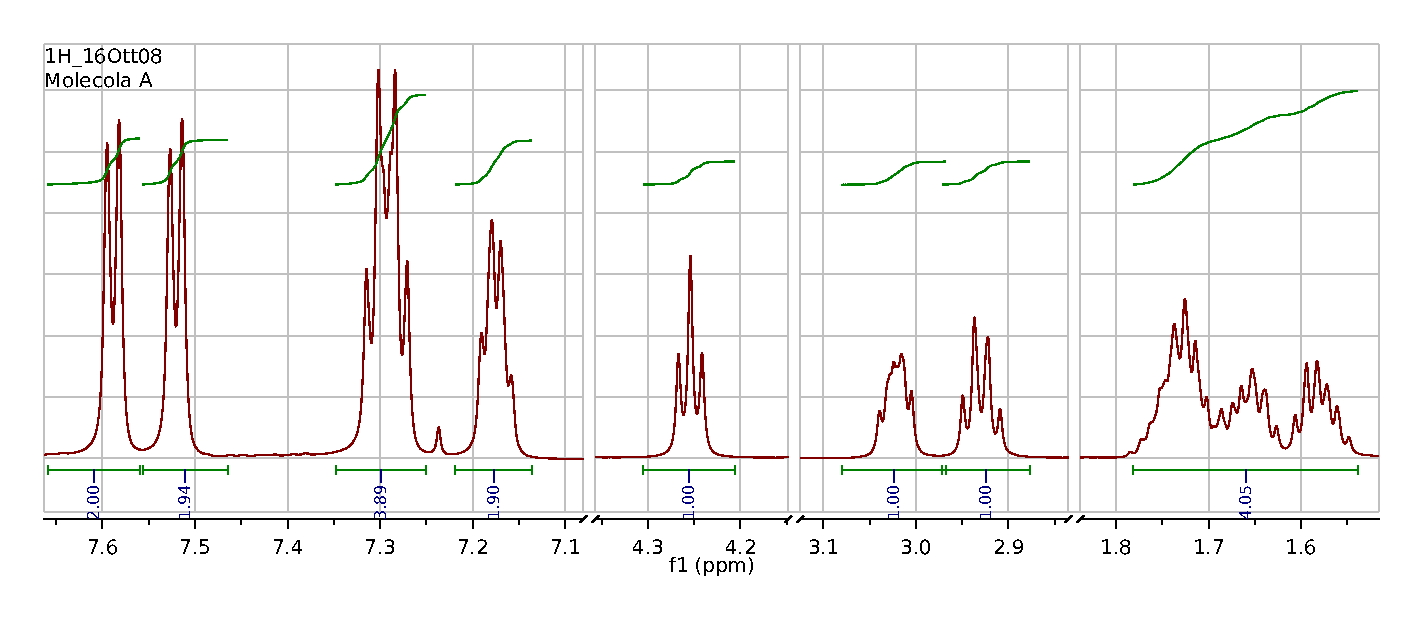
\includegraphics[height=0.7\textheight]{img/1hAc.pdf}\\\vspace{-20pt}
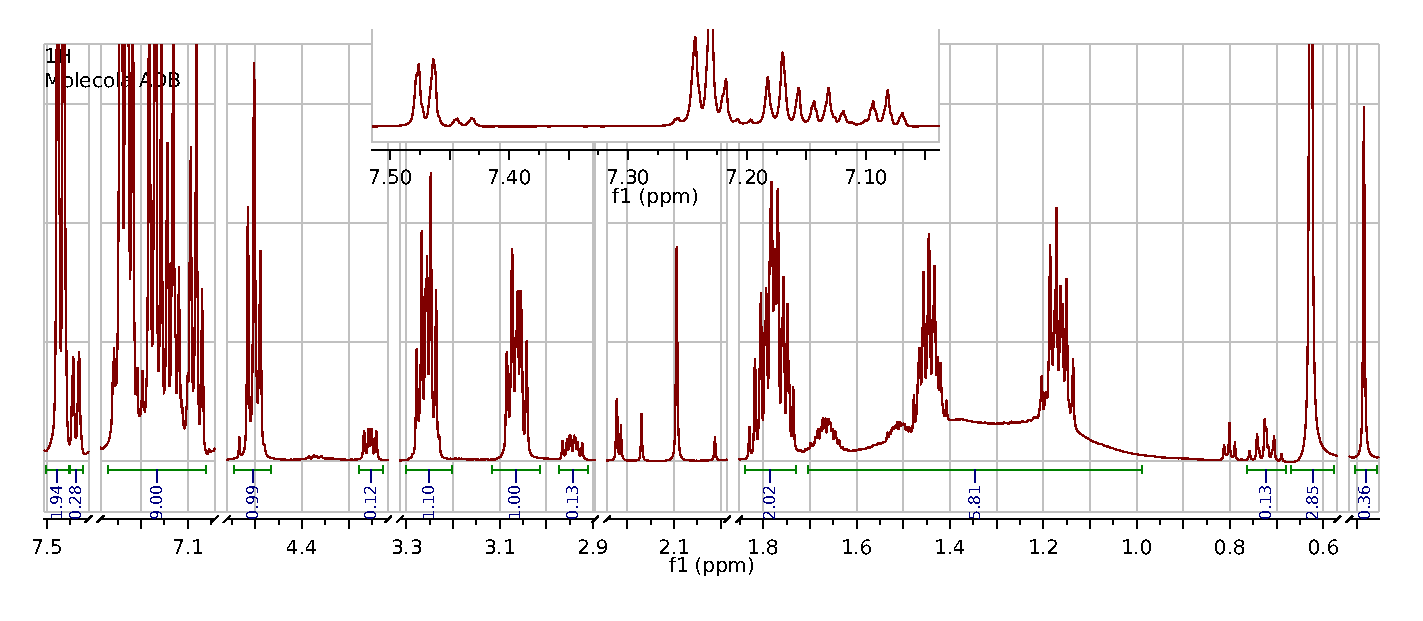
\includegraphics[height=0.7\textheight]{img/1hAOBb.pdf}
\end{figure}
\end{landscape}

\end{document}
